\documentclass[A4]{elsarticle}
\usepackage{graphicx}
\usepackage{amsmath}
\usepackage{amsfonts}
\sloppy

\begin{document}
\title{Test cases for the code Sky3D}

\author{Supplement to the manuscript ``{The TDHF Code Sky3D}''}
%\address{Institut f\"ur Theoretische Physik, Goethe-Universit\"at,
%  Max-von-Laue-Str. 1, \\60438 Frankfurt am Main, Germany}

\begin{abstract}
This directory {\tt Sky3D-Test} contains three simple examples for
running the code in its principal application modes: a static HF
calculation, a dynamic simulation of a giant resonance vibration
excited by an external field, and a collision between two nuclei.The
static case is used to provide the ground-state wave functions for
both time-dependent applications.
\end{abstract}

\maketitle
\section{Running the code}
The following instructions apply to a Linux system and the {\tt
  gfortran} compiler, but should be
quite similar for other Unix-based systems such as {\tt OS~X}.
In order to run the applications, the code must be compiled and linked
first by going into the code directory and then execute {\tt make} for
the standard version, {\tt make -f Makefile.openmp} for the {\tt
  OpenMP} version, and {\tt Makefile.mpi} for the {\tt MPI}
version. The executable program is named {\tt sky3d.seq}, {\tt
  sky3d.omp}, and {\tt sky3d.mpi}, respectively. Remember that MPI mode
works only for the dynamic case.

In the example directories there are input files {\tt for005.xxx} and
the standard output will go into {\tt for006.xxx}, where {\tt xxx} is
the name of the test case and the ``5'' and ``6'' were chosen as the
historic unit numbers for standard input and out in Fortran. Of
course, any other file name can be used instead.

{\bf A note on accuracy:} if the code is run on different computers,
the printed output will not be exactly identical due to differences in
round-off. The comparison of the results should take into account the
expected physical accuracy. For example, in the static calculation,
the dipole moments printed in {\tt dipole.res} should be zero; since
an {\tt E} format is used, the actual values show as numbers of the
order of $<10^{-15}$ with the digits essentially random. The same is
true, for example, for the $\gamma$ angle for a spherical nucleus
($\beta=0$), which is indeterminate but in practice results from small
inaccuracies in the quadrupole tensor components.  This
does in no way invalidate the results.

\section{The ground state of $^{16}$O}
The static calculation has to be run first to produce the ground-state
wave functions for the other test cases.
Going into the directory where the static case will be run, the command
line\\
\centerline{\em directory\tt/sky3d.seq < for005.static > for006.static  }
\\
with {\em directory} the directory where the code was compiled will
start the calculation. Of course the executable program can also be
copied or referred to by a symbolic link.

It produces a long protocol on 'for006.static' and a compact
one on 'conver.res'. The latter provides information on the most
basic observables as energy, energy convergence, energy variance,
radius and deformation. It does print these observables every {\tt
  mprint} times during iteration. The long output provides many more
details as, e.g., single-particle energies, again along the static
iteration. The most important output is the file 'O16' which
contains wave functions and fields from the ground state solution. This
will be used in the next step.  Note that the file name is set in the
input file {\tt for005.static}. A different name can be chosen; this
may be useful when running different test cases.

To verify correct execution, the contents of these files can be
compared with your own results and should agree within a reasonable
number of digits. Since the dipole moment of  $^{16}$O is zero, the
file {\tt dipoles.res} contains very small numbers with the digits
essentially random. The file {\tt spin.res} also shows only zeroes,
which in case should be reproduced, being printed in an ``F'' format;
the sign may be random, however.

The file {\tt conver.res} shows the typical behavior: the energy
converges quite rapidly, but the fluctuations take more iterations to
fall below the convergence limit. Since the deformation $\beta$ is
zero, the angle $\gamma$ has random values. If pairing is included and
for heavier nuclei the values for the fluctuations to not decrease as
much; often one has to live with the order of $10^{-4}$, whereas the
energy will still show nice convergence behavior.

In the output file {\tt for006.static} the properties of the
single-particle states should be noted. They show the correct
degeneracy and spin-orbit splitting with two nucleons in the
$1s_{1/2}$-state, which has zero orbital angular momentum, four
nucleons in the $1p_{3/2}$-state and two again in the
$1p_{1/2}$-state. For the $p$-states the angular momentum components
are not very instructive as there is no alignment. This is rarely
needed, but if necessary a diagonalization can be done in the
subspaces of degenerate states.

Note also that the proton states are pushed to somewhat higher
energies by the Coulomb force. 

The static calculation takes a few minutes on a modern PC.

\section{The quadrupole resonance in $^{16}$O}
\subsection{The physics case}

This is an example of how to initialize and study vibrational dynamics
of a nucleus, as outlined in section 2.5.3 of the documentation. The
test case deals with isoscalar quadrupole oscillations in  $^{16}$O and the
quadrupole resonance spectra deduced therefrom.

Giant resonances (GR) have for a long time been
prominent and much studied excitation modes of nuclei \cite{Goe82aR}.
Properly chosen Skyrme forces can provide a good description of them
\cite{Ben03aR,Klu09a}. As GR are related to nuclear dynamics, TDHF is
the correct starting point for their description. Traditional standard
is to use a linearized version of TDHF, called random-phase
approximation (RPA) \cite{Row70aB,Bro71aB}. This is extremely
efficient for spherical nuclei, but requires formidable formal
preparation, see e.g. \cite{Rei92a}. Conceptually much simpler and
numerically competitive for deformed nuclei is to use fully fledged
TDHF with subsequent spectral analysis \cite{Yab96,Cal97a}. This is
the line of development which we are following here. A detailed
discussion of spectral analysis of TDHF results is given in
\cite{Cal97a}. We report here only the practical steps for the given
example.

The present example considers the isoscalar quadrupole GR. It is
related to the isoscalar quadrupole operator
$\sum_n(2z_n^2-y_n^2-x_n^2)$ where $n$ runs over all nucleons, protons
and neutrons. The same operator couples to the excitation as well as
to the measurement. Actually, we will have to adapt the operator to a
periodic grid, see eq. (\ref{eq:quadgrid}). But this is a technical
detail. The quadrupole GR in heavy nuclei is a crucial benchmark for
the effective mass of nucleons in nuclei \cite{Boh79aR,Bar82a}. Our
example deals with a small nucleus for reasons of simplicity. It is
certainly an interesting exercise to extend the test to heavier
nuclei. We use for the example the Skyrme force SV-bas which is known
to reproduce the quadrupole GR in $^{208}$Pb fairly well
\cite{Klu09a}. It is also an interesting exercise to try the other
forces provided in the code.  Moreover, there are many other
interesting modes besides the isoscalar quadrupole GR, for example,
the isovector dipole GR or the isoscalar monopole GR
\cite{Boh79aR,Goe82aR}. One may also study these modes with the
present code. This is, however, a more sever exercise as the user has
to code the other multipole operators in {\tt external.f90}.

A word of caution is in order concerning the excitation spectrum at
low energies. The quadrupole spectrum for the present test case
$^{16}$O is nicely concentrated in the resonance region around 20
MeV. In heavier nuclei as, e.g., $^{208}$Pb, one will find also a low
lying peak in the range of a few MeV. These low lying parts of the
spectrum have to be taken with care for the case of non-magic nuclei.
The present code uses pairing at BCS level for stationary solution,
but freezes the pairing occupation numbers during the TDHF dynamics.
Effects from pairing dynamics would show up in the low-energy
spectrum. They are missing here and thus the low-energy part of the
spectrum cannot be trusted for open-shell nuclei. The GR region,
typically above 10 MeV, is not much affected by pairing and here we
can obtain still relevant results. An exception are closed-shell
nuclei (having $N,Z=$ 20, 28, 50, 82, 126, ...). Here, one can
trust the whole spectrum. Note, however, that a low-energy states
require high resolution which, in turn, needs long sampling times.


\subsection{Running the test case}
The dynamic calculation is executed by \\
%
\centerline{\em directory\tt/sky3d.seq < for005.dynamic > for006.dynamic} 
%
or the analogous command for the {\tt OpenMP} and {\tt MPI} cases,
where, again, you may discard the long output by redirecting it to
{\tt /dev/null} (because of the large size of the output file, this is
recommended in this case). The input file runs a dynamics which is
initialized by an instantaneous ('ipulse=0') boost. It is important
that we set 'texternal=T' in the input file to activate the
computation and use of a boost field. 

The file name for the one fragment in this case is given as {\tt
  ../Static/O16} to refer to the wave function file generated earlier
in the static run.

The boost operator is the isoscalar quadrupole. Note that we use a
quadrupole operator which is modified to comply with lattice
periodicity, i.e. we change
$x^2\Longrightarrow\sin(x*\pi/x_\mathrm{box})^2$ and similarly for y
and z where $x_\mathrm{box}$ is the $x$-extension of the box.  This
option is set by the {\tt textfield\_periodic=T} in the input file.
The Cartesian quadrupole then effectively reads
\begin{equation}
  \hat{Q}
  =
  2\sin\left(\frac{z\pi}{z_\mathrm{box}}\right)^2
  -\sin\left(\frac{y\pi}{y_\mathrm{box}}\right)^2
  -\sin\left(\frac{x\pi}{x_\mathrm{box}}\right)^2
\label{eq:quadgrid}
\end{equation}
which is close to the regular quadrupole in the vicinity of the nucleus
and bends to periodic shape towards the bounds of the box.  Now, it is
crucial to use just exactly the same operator in the spectral
analysis.  To that end, the corresponding expectation value of the
boost field $\hat{Q}$ is printed in the output file {\tt
  extfield.res}. We also take care to trigger only a small excitation
{\tt amplq0} to stay safely in the regime of linear response.  The
dynamical run will produce a couple of output files {\tt *.res}.  

Because the Fourier analysis need a large number of data and a long
physical duration of the calculation, the output is quite voluminous
and we provide only the most important files needed for the analysis:
{\tt energies.res} and {\tt extfield.res}. As the situation retains
spherical symmetry and the center of mass remains at rest, {\tt
  monopoles.res}, {\tt dipoles.res}, {\tt momenta.res}, and {\tt
  spin.res} contains zeroes or constant values. {\tt quadrupoles.res}
may warrant a brief look to see the oscillating quadrupole moments.

The running time will be several hours on a modern PC.

First, one should have a look at {\tt energies.res} and check that
conservation of particle number (columns 2 and 3) and energy (column
4) is fulfilled sufficiently well. A slight drift of the total energy
is unavoidable and acceptable. Any quick changes indicate numerical
problems. The run should then be discarded and another run with safer
numerical parameters should be performed.


Finally, we perform spectral analysis. To that end, we compile
the corresponding analyzing tool by\\
%
\centerline{\tt  gfortran spectral\_analysis.f90}
%
and execute it by\\
\centerline{\tt  ./a.out}
%
which produces two new output files. The routine reads the time
structure and the relevant quadrupole signal from {\tt extfield.res}.
It processes these data to produce spectra.  The output file {\tt
  extfield\_filt.res} contains a protocol of the filtered quadrupole
signals used in the spectral analysis. The file {\tt
  extfield\_spectrum.res} contains the spectral distributions. Its
column prints the frequency, columns 2-3 the (complex) Fourier
transform of the filtered isoscalar quadrupole signal, where its
imaginary part (column 3) is identified as being proportional to the
quadrupole strength. Column 4 shows the absolute squared of the
Fourier transform which is the spectral power.

\subsection{Results for the test case $^{16}$O}

\begin{figure}
\centerline{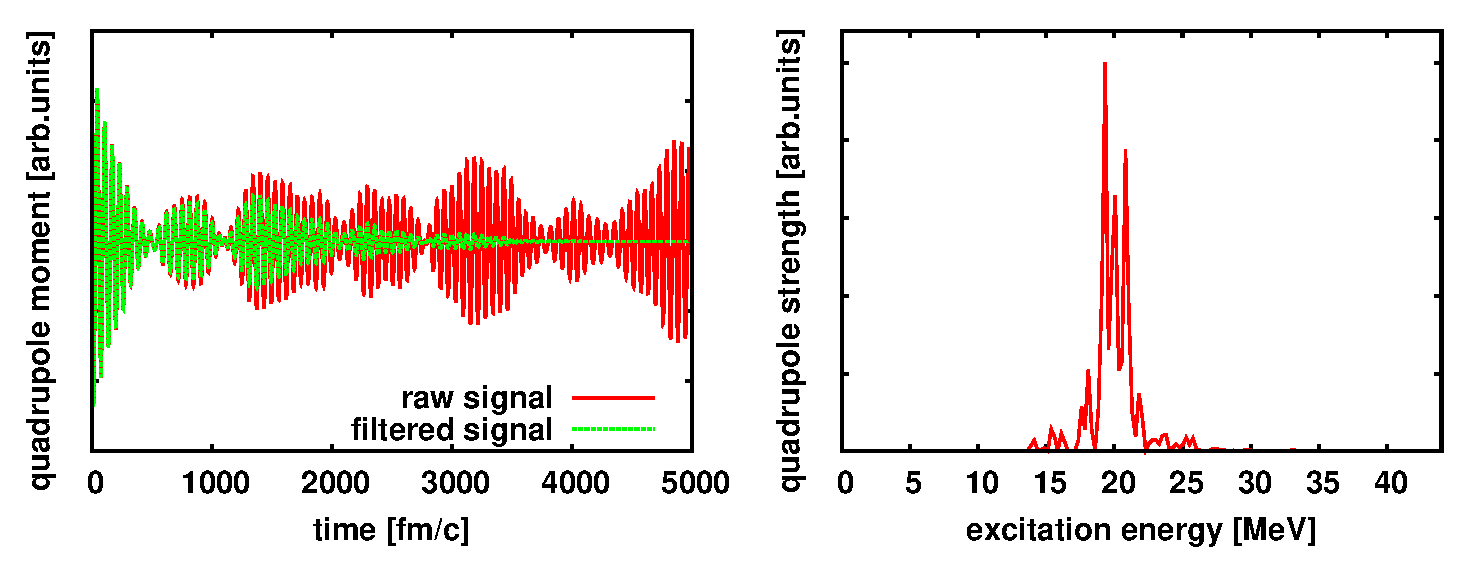
\includegraphics[width=\linewidth]{testcase-16O.eps}}
\caption{\label{fig:testcase-16O}
The quadrupole signal in the time domain (left) and frequency
domain (right) for the present test case of quadrupole oscillations
in $^{16}$O computed with the forces SV-bas. Note that frequency is
converted to excitation energy by $E_\mathrm{esc}=\hbar\omega_\mathrm{exc}$.
}
\end{figure}
The example on the actual file {\tt extfield\_spectrum.res} contains
the result of a calculation up to time 5000 fm/c.  Its content is
shown as the curve ``raw signal'' in the left panel of figure
\ref{fig:testcase-16O}. The ``filtered signal'' on the same panel is
taken from the file {\tt extfield\_filt.res}. One sees how filtering
suppresses the signal strongly towards the end of the sampling
interval. The long sampling time of 5000 fm/c provides an energy
resolution of about 0.3 MeV, more than enough for displaying a giant
resonance. The right panel of figure \ref{fig:testcase-16O} shows the
spectral quadrupole strength as found in the file {\tt
  extfield\_spectrum.res} (column 3 versus column 1). The strength is
nicely focused in one resonance region but rather fragmented over
several sub-peaks. The overall resonance position is a relevant
feature. However, the detailed fragmentation is not to be taken
seriously as it is strongly affected by the finite numerical box. The
resonance energy resides actually in the nucleon continuum. Thus the
detailed structures should be washed out much more by line broadening
through particle emission. The present fine structure is an artifact
from the computational box.  Emission effects can only be described by
using absorbing boundary conditions \cite{Rei06a}. A simple solution
to broaden the signal for the present code is to use stronger
filtering (enhance {\tt nfilter} in {\tt spectral\_analysis.f90}).

\section{Collision of $^{16}$O+$^{16}$O}
\subsection{The physics case}
The use of TDHF for the description of heavy-ion collisions goes back
to the beginning of this field.Its strong points are that is provides
a natural description of neck formation and rupture between two nuclei
and allows the full spectrum of collision behavior: fusion,
deep-inelastic collisions, grazing collisions, even multifragmentation
\cite{simenel}. The omission of nucleon-nucleon collisions, however,
prevents complete equilibration \cite{loebl}, and for this reason it
should not be applied to study the long-term behavior, e.~e., of a
compound nucleus. Here we selected a relatively simple scenario of two
$^{16}$O nuclei colliding at 100~MeV of relative-motion kinetic energy
and an impact parameter of 2~fm. This is a deep-inelastic collision.

\subsection{Running the test case}
The dynamic calculation is executed by \\
%
\centerline{\em directory\tt/sky3d.seq < for005.dynamic > for006.dynamic} 
%
or the analogous command for the {\tt OpenMP} and {\tt MPI} cases.
The input file describes initialization for two fragments ({\tt
  nof=2}) and in the {\tt NAMELIST} {\tt fragments} both refer to the
same wave function file {\tt ../Static/O16}. It also determines the
kinetic energy and impact parameters for a two-body initialization
({\tt fix\_boost=.FALSE.}). Finally the center-of-mass positions of
the fragments are given.

\subsection{Results}
A check of the file {\tt energies.res} shows that the particle number
is preserved to about 0.01\%. The energy stays constant within about
one MeV and the agreement of integrated and summed energies is also at
that level of accuracy. The collective energies go down significantly,
however, showing that this indeed a deep-inelastic collision. Note the
different physical meaning: {\tt Ekin} is the expectation value of the
kinetic energy operator, which includes both the energy associated
with probability flow as well as that due to localization of the wave
functions. {\tt Ecoll}, on the other hand, is only the energy
associated with the average flow, which contains, however, the
internal collective motion of the nuclei. Under the influence of the
Coulomb field the protons and neutrons behave slightly differently.

The file {\tt dipoles.res} only shows that the dipole moment of the
complete system remains practically zero. In {\tt monopoles.res} the
r.m.s\ radii are quite useful; especially the total r.m.s. radius can
be taken as a measure for the separation which goes over into a
deformation coordinate when the nuclei coalesce. {\tt momenta.res}
shows that the center of mass of the total system remains at rest,
while the data in {\tt quadrupoles.res} are less interesting in a
collision. The file {\tt spin.res} indicates a reasonable conservation
of angular momenta but some exchange between orbital and spin
contributions. 

Finally the output file {\tt for006.coll}is useful in many ways. The
regularly produced printer plots give a good indication of what is going
on without needing the effort of converting the file format and
starting up a visualization code. It is often helpful to look at the
initial printer plots while the code is running in order to see
whether things are working as planned.

The ``relative motion'' and ``collision kinematics'' printout is also
very useful, although it is produced only if a two-body situation is
recognized, i.~e., not during the interaction phase. From the first
analysis seen it is clear that neither the relative energy nor the
angular momentum are reproduced very precisely. One reason is that
cutting up space into two halves assigns a non-negligible part of each
nucleus to the other side and distorts the results somewhat. If higher
accuracy is desired, it would be better to separate the system into the
two original sets of wave functions, but while this can be used to
correct the initial setup, it cannot be applied to the final state,
where wave functions extend over both fragments.

If you ``grep'' the output file for ``ecmf'', a short overview of the
development of the orbital angular momentum and the final center-of-mass
energy is produced. The energy decreases from 100~MeV to about 18~MeV,
but does not approach a true constant. This has two principal reasons:
the separated nuclei still  show collective oscillations which are
coupled to the Coulomb field, and also the unphysical effect of
wave functions crossing the boundary may play a role \cite{guo}. 
 If these should prove critical, measures such as
absorbing potentials on the boundary may have to be invoked
\cite{absorb}.

The angular momentum calculated in the two-body analysis shows much
stronger fluctuations than the quantum-mechanical one printed in {\tt
  spin.res}. The latter shows an almost constant total angular
momentum with only a small exchange between spin and orbital
contributions. This indicates that some angular momentum is in
internal excitation of the fragments,

The collision calculation takes several hours on a modern PC.

\begin{thebibliography}{99}

\bibitem{Goe82aR}
K. Goeke and J. Speth,
% title    = "Theory of giant resonances", 
Ann. Rev. Nucl. Part. Sci. {\bf 32}, 65 (1982).


\bibitem{Ben03aR}
M.~Bender, P.H. Heenen, P.G. Reinhard, Rev. Mod. Phys. \textbf{75}, 121 (2003),
  \texttt{http://dx.doi.org/10.1103/RevModPhys.75.121}

\bibitem{Klu09a}
P.~Kl\"upfel, P.~G.~Reinhard, T.~J.~B\"urvenich, J.~A.~Maruhn, Phys.Rev. 
  C\textbf{79}, 034310 (2009), http://www.arxiv.org/abs/0804.3385,
  \texttt{http://link.aps.org/doi/10.1103/PhysRevC.79.034310}


\bibitem{Row70aB}
{D.~J.~Rowe}, {\emph Nuclear Collective Motion}, 
({Methuen}, {London}, {1970})


\bibitem{Bro71aB}
G.~E.~Brown, \emph{Unified Theory of Nuclear Models and Forces}, 3rd~edn.
  (North-Holland, Amsterdam, London, 1971)


\bibitem{Rei92a}
%title={{RPA} in wavefunction representation},
P.-G.~Reinhard and Y.~Gambhir,
{Ann. Phys. (Leipzig) } {\bf 504}, 598 (1992);
\\
%title={From sum rules to {RPA}: 1. Nuclei},
{P.-G.~Reinhard},
{Ann. Phys. (Leipzig) } {\bf 504}, 632 (1992).


\bibitem{Yab96}
K.~Yabana and G.~F.~Bertsch,
Phys. Rev. B{\bf 54}, 4484 (1996).

\bibitem{Cal97a}
F.~Calvayrac, E.~Suraud, P.-G.~Reinhard, Ann. Phys. (N.Y.) \textbf{255}, 125
  (1997), \texttt{http://dx.doi.org/10.1006/aphy.1996.5654}


\bibitem{Boh79aR}
O.~Bohigas, A.~M.~Lane, and J.~Martorell, 
% title   = {Sum Rules for Nuclear Collective Excitations}, 
Phys. Rep. {\bf 51}, 267 (1979).

\bibitem{Bar82a}
J.~Bartel, P.~Quentin, M.~Brack, C.~Guet, H.B. H{\aa}kansson, Nucl. Phys.
  A\textbf{386}, 79 (1982)

 
\bibitem{Rei06a}
%  title={Role of boundary conditions in dynamic studies of nuclear giant resonances},
P.--G.~Reinhard, P.~D.~Stevenson, D.~Almehed, J.~A.~Maruhn, and M.~R.~Strayer,
{Phys. Rev. E}{\bf 73}, 036709 (2006).

\bibitem{simenel}
C.~Simenel, E.P.J. A{\bf 48}, 1 (2012).

\bibitem{loebl}
N.~Loebl, J.~A.~Maruhn, and P.-G.~Reinhard,  Phys. Rev. C\textbf{84}, 034608 (2011).

\bibitem{guo}
Lu~Guo, P.-G.~Reinhard, and J.~A.~Maruhn,
Phys.~Rev. C{\bf 77}, 041301 (2008).

\bibitem{absorb}
P.-G.~Reinhard, P.~D.~Stevenson, D.~Almehed, J.~A.~Maruhn, and M.~R.~Strayer,
Phys.~Rev. E{\bf 73}, 036709 (2006).
\end{thebibliography}

\end{document}
